%!TEX root = ../thesis_phd.tex
%%%%%%%%%%%%%%%%%%%%%%%%%%%%%%%%%%%%%%%%%%%%%%%%%%%%%%%%%%%%%%%%%%%%%%%%%%%%%%%%
% reconstruction.tex:
%%%%%%%%%%%%%%%%%%%%%%%%%%%%%%%%%%%%%%%%%%%%%%%%%%%%%%%%%%%%%%%%%%%%%%%%%%%%%%%%
\chapter{Event Reconstruction}
\label{reconstruction_chapter}
%%%%%%%%%%%%%%%%%%%%%%%%%%%%%%%%%%%%%%%%%%%%%%%%%%%%%%%%%%%%%%%%%%%%%%%%%%%%%%%%

In order to extract useful physics information from the \nova detector, the raw
data (cell hits) must be processed into higher level forms.
This processing step is known as reconstruction.
For this analysis, the primary goals of reconstruction are to identify \numu
charged-current (CC) interactions and estimate the energy of the neutrinos involved in the interactions. Identification of \numu CC interactions is really
a task of rejecting backgrounds induced by both cosmic rays and the \numi beam.  The cosmic ray background dominantly composed of down-going muons,
although other particles can also be present.  Backgrounds in the \numi beam
include both neutral current (NC) interactions and CC interactions from \nue or
\nutau.

Traditional reconstruction efforts involve detection of lines and other shapes
in raw data.  Classification is then a process of extracting manually
engineered features from those events which discriminate between signal and
background.
This analysis uses machine learned features in a convolutional neural network
to replace manual feature engineering.
The approach presented here differs in that the hits themselves are presented
to the neural network as two separate images, corresponding to $x$ (vertical)
and $y$ (horizontal) views.
The goal with this approach is to sidestep pathological failures incurred in each reconstruction and feature engineering step, thus allowing more of those pathological events to be more correctly classified.

The \nova \textit{event display} provides a visualization of the raw detector readout which serves as the input to reconstruction.
An example event display is shown in figure \ref{eventDisplay14}.
The data corresponds to 550 $\mu s$ of Far Detector (FD) readout, with hits colored according to their time recorded relative to the start of the readout window.
Visible activity displayed falls into two primary groups: randomly distributed electronic noise and correlated activity from cosmic rays.
Since cosmic rays cross the detector quickly, hits along each track are displayed as a uniform color.

\begin{figure}[t]
\begin{center}
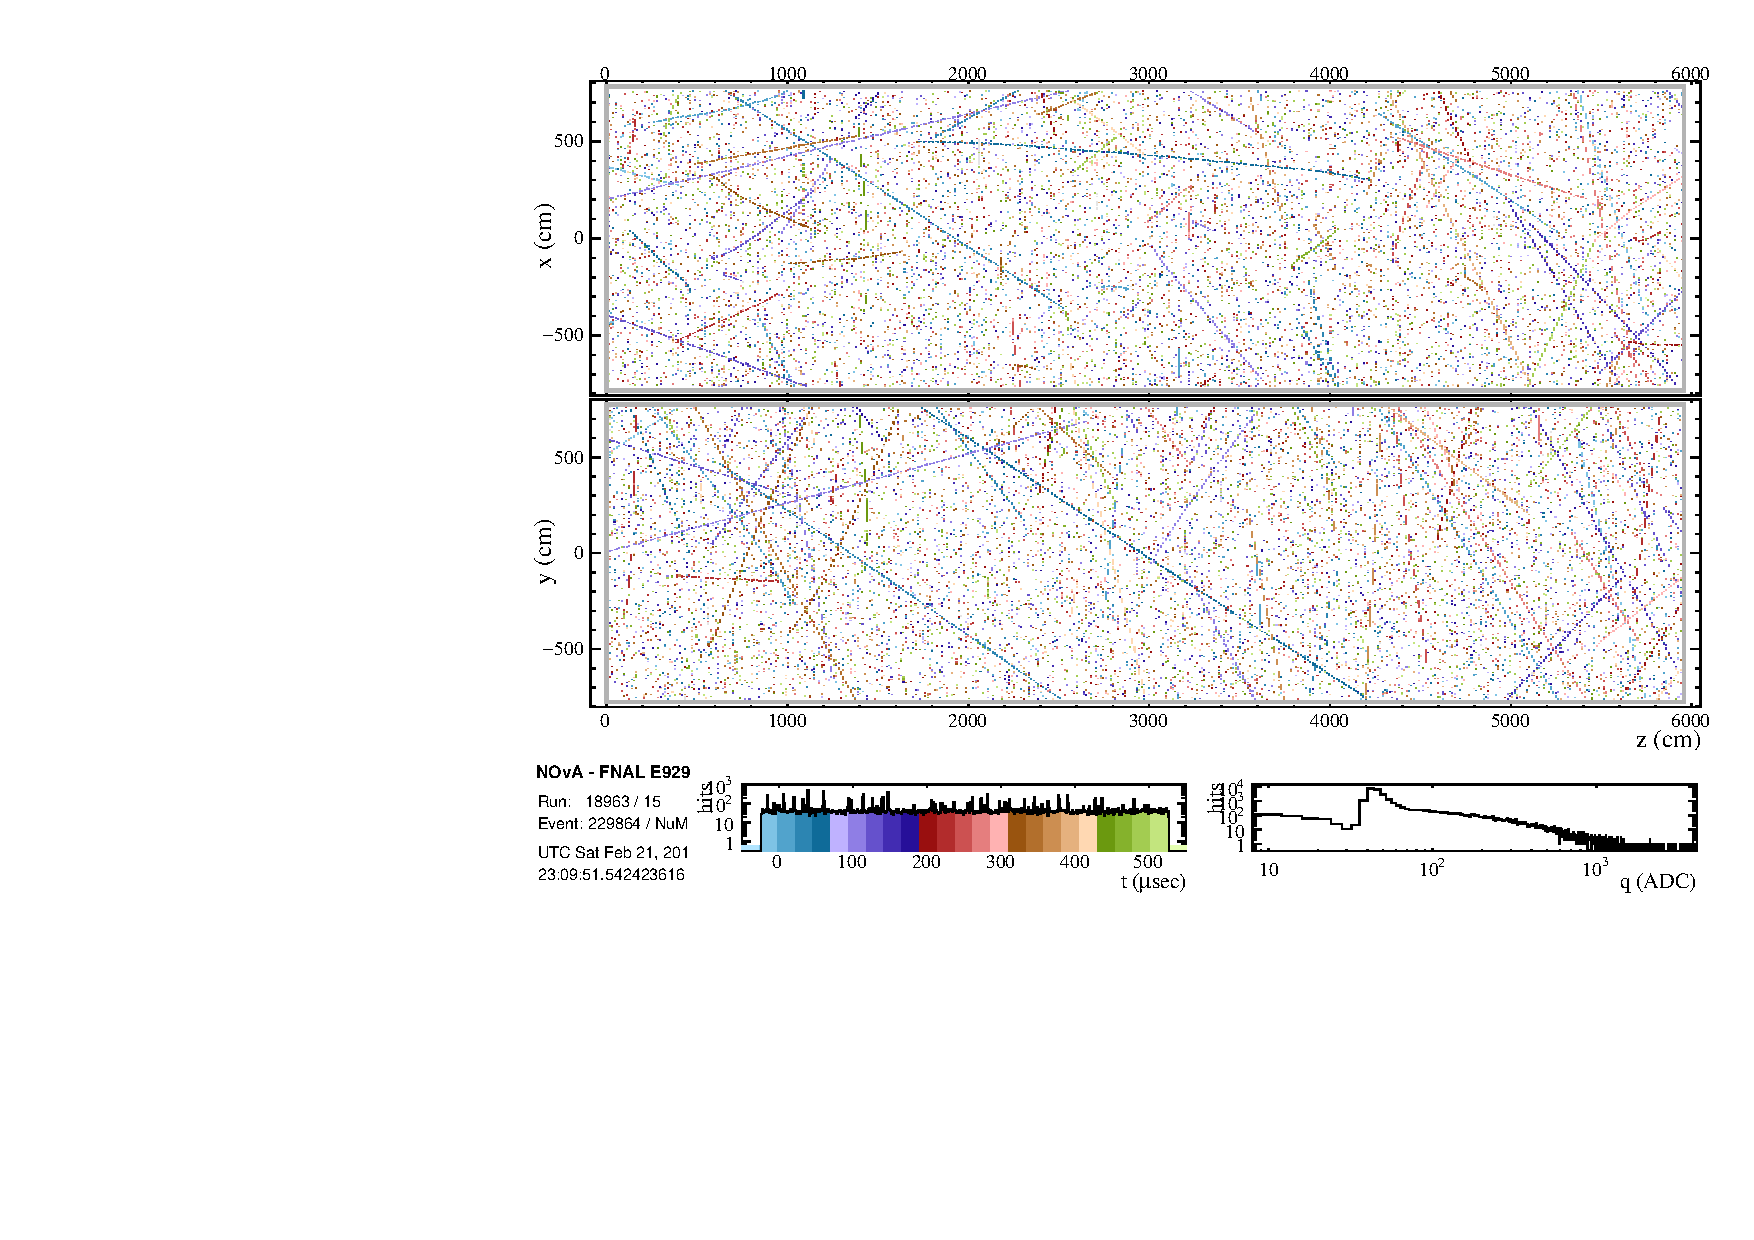
\includegraphics[width=\textwidth]{figures/evd/evd_14db.pdf}
\end{center}
\caption{An example \nova event display.  The top projection is an $x$ vs. $z$ view, the bottom is $y$ vs. $z$.  Hits are colored by the at which they were recorded relative to the start of the readout window; the color scale is visible in the bottom center pane.}
\label{eventDisplay14}
\end{figure}

\section{Slicing}

The first task in reconstructing \nova data is to resolve individual particle interactions

\section{Tracking}

\subsection{Least-squares Regression}

We fit lines to regions of tracks.


\subsection{Kalman Filtering}

We expand tracks from pairs based on chi-square.

\section{Calibration}

An important input to many reconstruction efforts is an accurate estimate of
the energy deposited in a cell.  Calibration procedures aim provide an the
estimation of energy deposition based on the recorded ADC value and position
of a particular cell hit.  The \nova calibration accounts for three primary
effects: attenuation
of light in the wavelength shifting fiber, cell-to-cell variations, and
conversion conversion from ADC scale to physical energy units.

\subsection{Attenuaiton and Cell-to-cell Corerection}

The attenuation correction is based upon cosmic ray muons since they are
abundant and their energy deposition properties are well understood.  A
reference sample of cell hits is selected from muon tracks which satisfy a few
simple characteristics.  First, tracks must touch two detector faces,
indicating that they traversed the detector rather than stopping inside.  The
tracks are required to cross at least ten planes to ensure that path length
(distance traversed by the muon within each cell) can accurately be estimated.
Hits on selected tracks are only used for calibration if they satisfy the
so-called tri-cell criterion; that is, that there are also hits present in
adjacent planes.  This criterion also helps ensure that a reasonable path
length estimate is obtained.  Certain cells fail to produce enough its to allow
the subsequent attenuation fits to be obtained, for instance cells on the edges
of the detector and those adjacent to dead cells.  Such cells are calibrated
with alternative samples with hits in adjacent cells.

\begin{figure}[t]
\begin{center}

\includegraphics[width=0.7\textwidth]{figures/dummy/dummy.jpg}
\end{center}
\caption{NEED TO GET THE RIGHT PLOT HERE... attenuation PE/path length vs. W.}
\label{calib_atten}
\end{figure}

For each reference hit, the ADC value is converted to PE based on a scale
factor.  The path length and position along the cell (i.e. distance from the
APD readout) are both estimated from the muon track trajectory.
A 2D histogram of the ratio of PE to path length vs. position along cell is
constructed for each cell.
A fit is to the mean PE per path length response function of
position is used to characterize each cell.
The functional form for the middle part of the cells is a sum of two
exponentials, one corresponding the short trip to the APD and the other for
the long way to the far end of the cell and back around the fiber loop.
\begin{equation}
y(W) = C + \bigg ( \exp \big( \frac{W}{X}\big) +
\exp \big( - \frac{L + W}{X}\big)  \bigg )
\end{equation}
Above, $W$ is the position along the cell, $X$ is the fiber attenuation length,
and $L$ is the length of the cell.
The attenuation length as well as constants $C$ and $A$ are free parameters
in the fit.
At the end of cells, a diminished response known as \texit{roll-off} has been
observed, presumedly due
to light being absorbed at the ends rather than in the fiber.
The deficit of light is empirically well described by an $x^4$ form
\begin{equation}
  y=\left\{\begin{tabular}{cl}
    $1-\alpha_R(x-x_R)^4$ & $x>+x_R$\\
    1 & otherwise\\
    $1-\alpha_L(x-x_L)^4$ & $x<-x_L$
  \end{tabular}\right.
  \label{eqn:rolloffs}
\end{equation}
where free parameters $x_R$ and $x_L$ indicate the start of the roll-off
region on either side and $\alpha_R, \alpha_L$  determine the scale.

From the attenuation fits, a hit at any position can be corrected to a
baseline value.
The centers of the cells are all pinned to the same baseline, which effectively
removes cell-to-cell variations.

\subsection{Absolute Energy Calibration}

This is the next step!

\begin{figure}[t]
\begin{center}
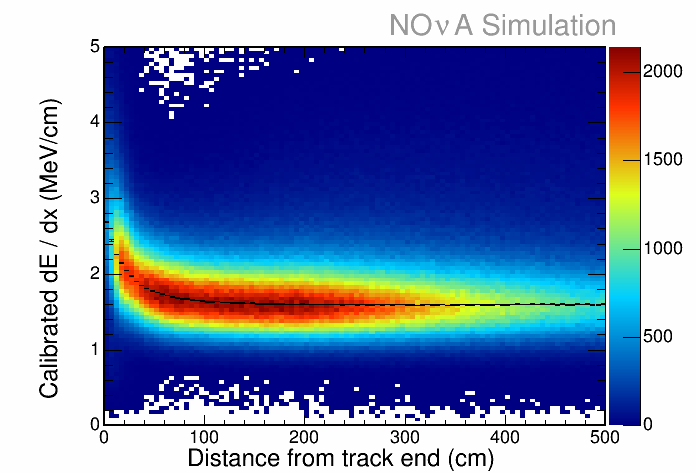
\includegraphics[width=0.8\textwidth]{figures/plots/reco/calib_dEdX.png}
\end{center}
\caption{2D histogram depicting deposited energy per path length (dE/dX) for
cell hits after attenuation and cell-to-cell correction.  Color scale
indicates the number of measurements in each bin.  The rise in energy at the
end of muon track (left) is well described by the Bethe-Bloch formula \cite{pdg}.}
\label{calib_dEdX}
\end{figure}

\section{Image Formation}

\section{Architecture and Training}

We use siamese googlenet, two googlenets side-by-side

We train first for all event types



%%%%%%%%%%%%%%%%%%%%%%%%%%%%%%%%%%%%%%%%%%%%%%%%%%%%%%%%%%%%%%%%%%%%%%%%%%%%%%%%
